\section{CSR Game Model}\label{sec:game-model}

In this section we introduce the capacitated selfish replication (CSR) game with binary preferences as was introduced in \cite{gopalakrishnan2012cache}. 

We start with a set of $[n]=\{1,2,\ldots,n\}$ nodes (players) which are connected by an undirected graph $\mathcal{G}=([n], \mathcal{E})$, and a set of all resources denoted by $O=\{o_1, o_2,\ldots, o_k\}$. We assume that each node has access to all the resources, but due to the capacity constraint it can hold only one resource in its cache. For a particular allocation $P=(P_1, P_2, \ldots, P_n)$ with $P_i\in O$, we define the sum cost function $C_i(P)$ of the $i$th player associated with this  profile as follows:
\begin{align}\label{eq:CSR-cost-formulation}
C_i(P)=\sum_{o\in O\setminus \{P_i\}}d_{\mathcal{G}}(i, \sigma_i(P,o)), 
\end{align}
where $\sigma_i(P,o)$ is $i$'s nearest node holding $o$ in $P$. Moreover, we let $\mathcal{P}$ be the set of all possible allocation profiles. In Figure \ref{fig:example-model} we have illustrated an instance of the CSR game for $n=11$ and $|O|=3$, and provided the associated costs for two players $i=1,8$.

\begin{figure}[htb]
\vspace{-1.5cm}
\begin{center}
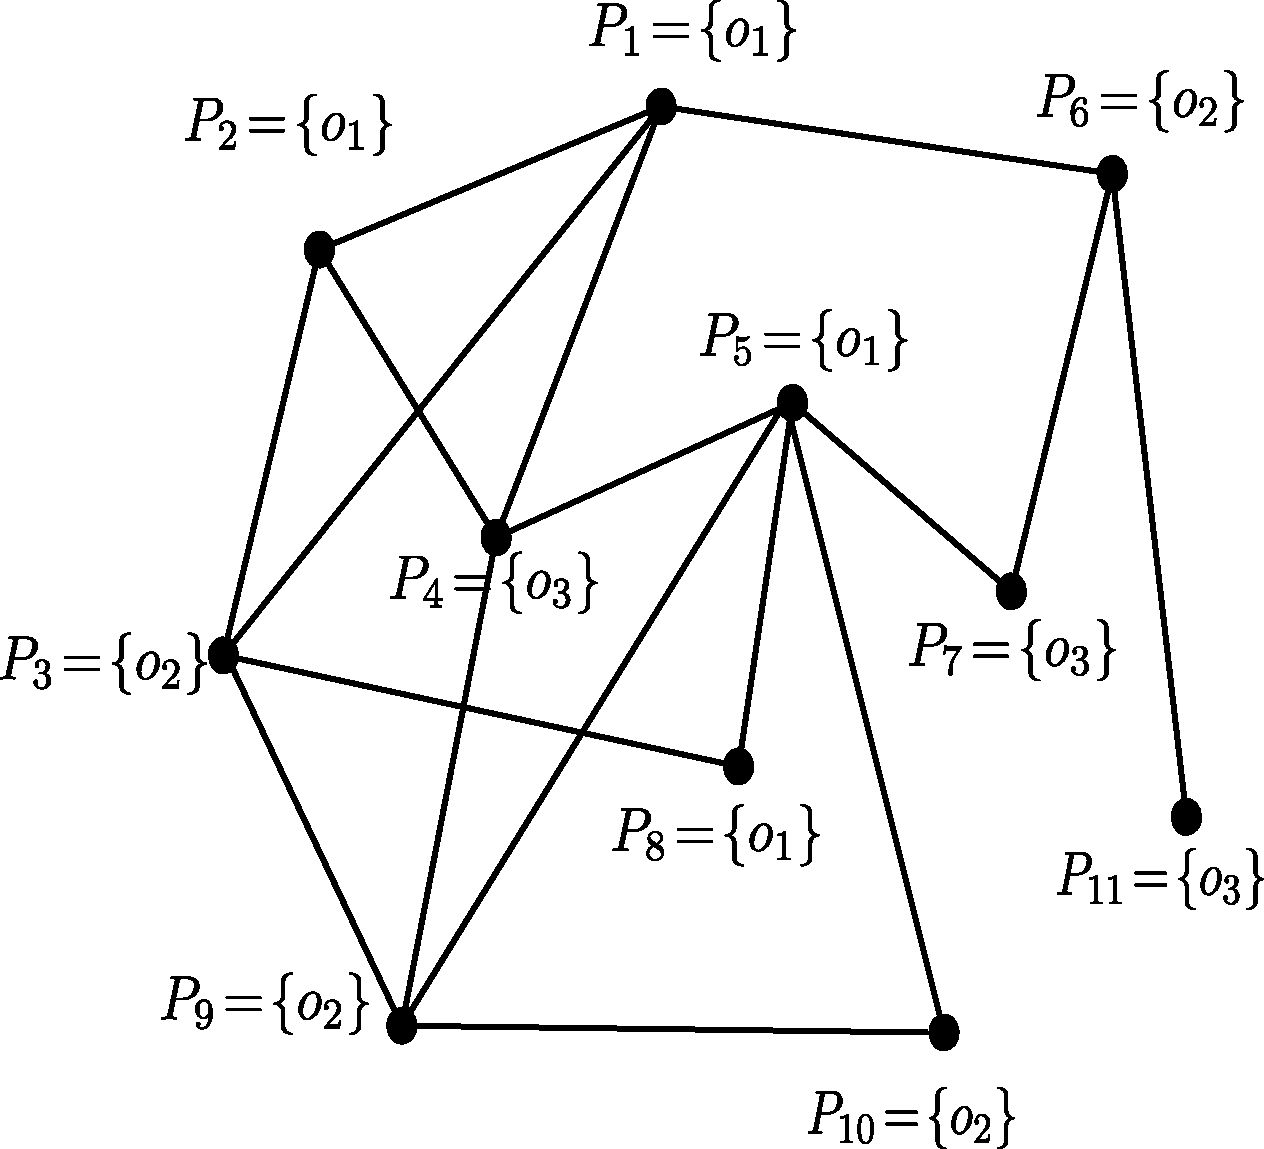
\includegraphics[totalheight=.22\textheight,
width=.4\textwidth,viewport=-50 0 800 750]{example} \hspace{0.4in}
\end{center}
\vspace{-0.3cm}\caption{CSR game with $n=11$ players and $O=\{o_1,o_2,o_3\}$ resources. We have $C_1(P)=0+1+1=2, C_8(P)=0+1+2=3$ and $r_1(P)=1, r_8(P)=1$.}
\label{fig:example-model}
\end{figure}
\vspace{-0.3cm}
\begin{remark}
If some resource $o$ is missing in an allocation profile $P$, we define the cost of each player for that specific resource to be large, e.g., $d_{\mathcal{G}}(i, \sigma_i(P, o)) = n, \forall i \in [n]$. Therefore, for $n \ge |O|$, this incentivizes at least one of the players to allocate the missing resources in the network. In the case where $n < |O|$, all the players will allocate different resources and the game becomes trivial, hence we can simply assume that $n \ge |O|$. 
\end{remark}

%\begin{remark}\label{rem:varying-cache}
%Actually all the proofs in this paper can be carried over to games with varying capacities by constructing a new network which transfers games with different cache sizes to one with unit size caches \cite{etesami2014pure,gopalakrishnan2012cache}.
%\end{remark}

\begin{definition}
An allocation profile $P^*$ is said to be a pure-strategy Nash equilibrium of the CSR game if 
\begin{align}\nonumber
C_i(P^*_i,P^*_{-i})\leq C_i(P_i,P^*_{-i}), \ \forall i\in[n], \forall P_i\in O.
\end{align}
where $P^*_{-i}$ denotes the cache content of all the players other than the $i$th player.
\end{definition}

It has been shown in \cite{gopalakrishnan2012cache} that the CSR game has an associated ordinal potential function, and hence, it has at least one pure Nash equilibrium. More precisely:

\begin{theorem}\label{thm:existence-NE}
The CSR game admits an ordinal potential function, and hence, a pure-strategy Nash equilibrium.
\end{theorem}

Although Theorem \ref{thm:existence-NE} proves the existence of NE, however, in general it can only guarantee an exponential number of iterations $\mathcal{O}(|O|^n)$ for finding such equilibrium points. Therefore, the main challenge here is to find an efficient way to arrive at an equilibrium which we will address in the remaining of this paper.
